Parameters affecting the bandgap energy shifts in argon
plasma-induced quantum well intermixing have previously been studied
in detail elsewhere \cite{icpparam}. Inductively coupled plasma
(ICP) parameters, RTA parameters and QW layer structure are three
main factors affects the magnitude of bandgap energy shifts. In my
experiments, ICP and RTA parameters were investigated.

\begin{table}[!t]
    \renewcommand{\arraystretch}{1.3}
    \caption{The layer structure for the 0.9\% compressive strain
        InGaAsP/InGaAsP multiple quantum well}
    \centering
    \label{mySample}
    \begin{tabular}{cccc}
        \hline
        \hline
        Layer & Composition & Thickness(nm) & Doping(cm$^{-3}$)\\
        \hline
        Sacrificial & InP                          & 500  & Zn\\
        Cap         & p$^+$-InGaAs                 & 200  & Zn:1e19\\
        Cladding    & p-InP                        & 1500 & Zn:1e18\\
        Etch-stop   & p-InGaAsP (1.24um)           & 10   & Zn:4e17\\
        Cladding    & p-InP                        & 150  & Zn:4e17\\
        GRINSCH     & p-InGaAsP (1.05um)           & 20   & Zn:4e17\\
        GRINSCH     & p-InGaAsP (1.15um)           & 20   & Zn:4e17\\
        GRINSCH     & p-InGaAsP (1.24um)           & 20   & Zn:4e17\\
        QW                 & InGaAsP               & 5    & $-$\\
        Barrier$\times$7   & InGaAsP (1.24um)      & 10   & $-$\\
        QW$\times$7        & InGaAsP               & 5    & $-$\\
        GRINSCH     & p-InGaAsP (1.24um)           & 20   & Si:4e17\\
        GRINSCH     & p-InGaAsP (1.15um)           & 20   & Si:4e17\\
        GRINSCH     & p-InGaAsP (1.05um)           & 20   & Si:4e17\\
        Buffer      & n-InP                        & 1500 & Si:2e18\\
        Substrate   & n$^+$-InP                    & $-$  & S or Sn:~4e18\\
        \hline
        \hline
    \end{tabular}
\end{table}
The layer structure of the QW samples is shown in Table
\ref{mySample}. The plasma source generator used in the experiments
was a Plasmalab System 100, which was built by Oxford Instruments.
The ICP parameters were optimized using 80-sccm Ar flow rate,
80-mtorr chamber pressure, 480-w RF power, 500-w ICP power,
20$^\circ$C temperature, 1-min time. After Ar plasma exposure, the
samples were annealed at 600$^\circ$C-800$^\circ$C for 2 min in a
rapid thermal processer (RTP) in a nitrogen atmosphere. Two fresh
pieces of InP were used to provide an phosphorous over-pressure
environment during the annealing process and further to prevent the
sample surface from phosphorous outdiffusion. Room-temperature (RT)
Photoluminescence (PL) measurements were then performed to obtain
the bandgap energy shifts data.

\begin{figure}[!t]
    \centering
    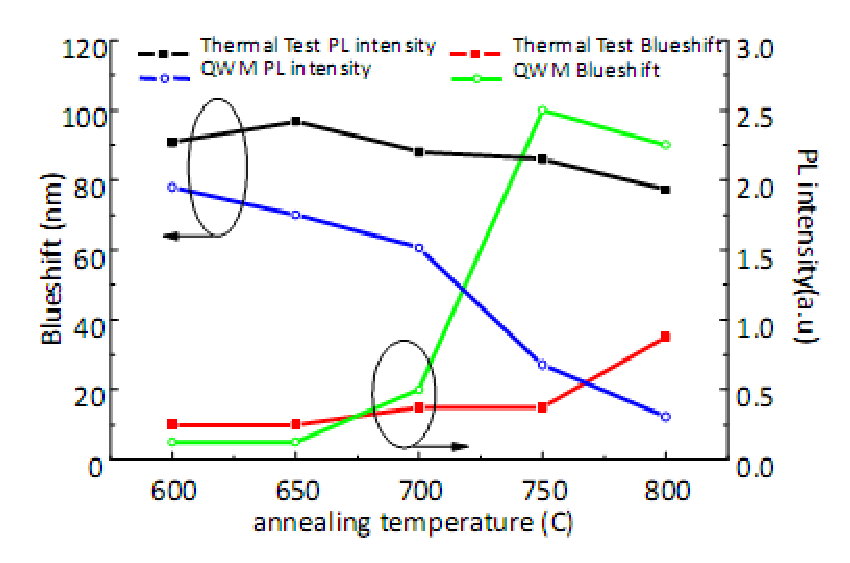
\includegraphics[width=2.5in]{fig/rta1}
    \caption{Bandgap blue shift and PL peak intensity vs. RTA temperature}
    \label{ex_rta1}
\end{figure}
Figure \ref{ex_rta1} shows the bandgap blue shift and PL peak
intensity in different RTA temperature. Large bandgap shift of
\~90nm is obtained under RTA temperature of 750$^\circ$C, while the
PL peak intensity decrease of 80\% is slight and acceptable.

\begin{figure}[!t]
    \centering
    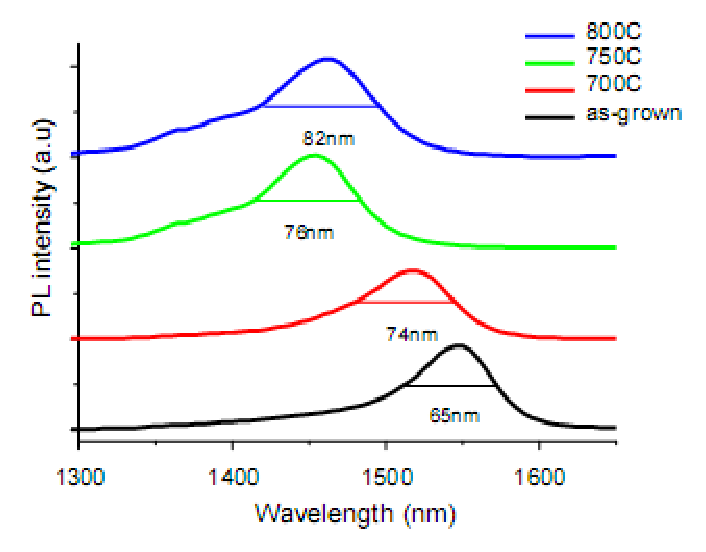
\includegraphics[width=2.5in]{fig/rta2}
    \caption{PL vs. wavelength}
    \label{ex_rta2}
\end{figure}
Figure \ref{ex_rta2} shows the full width at half maximum (FWHM) of
the PL under different RTA temperature. The slight linewidth
broadening may result from different bandgap blue shift of TE and TM
modes of the PL.
